\chapter{Mechanizm zabezpieczaj�cy przed uszkodzeniem stanowiska}

W celu zabezpieczenia stanowiska przed przepe�nieniem zbiornik�w (tj. $H1$ lub $H2$ lub $H3$ osi�gnie warto�� $\num{20}$) zaimplementowano poni�ej przedstawiony (rys. \ref{safety_mechanism_code_t}) mechanizm zabezpieczaj�cy.

\begin{figure}[h!]
	\centering
	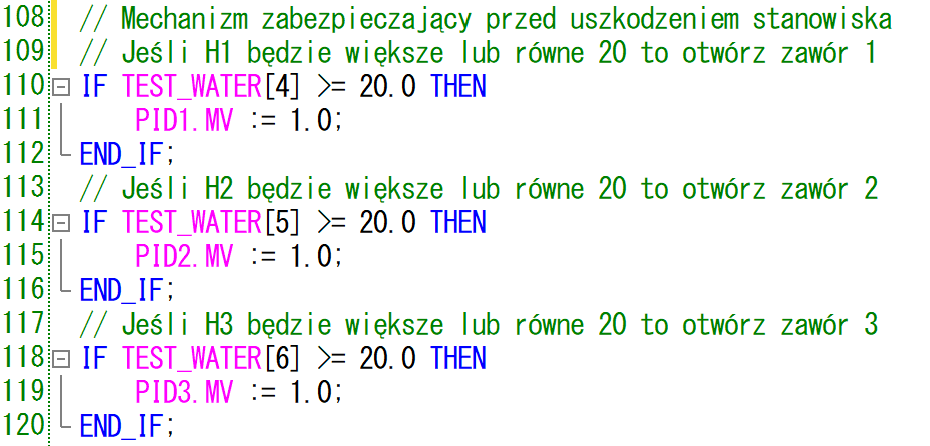
\includegraphics[width=\textwidth, center]{rysunki/SAFETY_MECHANISM_CODE_T.png}
	\caption{Kod zabezpieczaj�cy przed uszkodzeniem stanowiska ze zbiornikami}
	\label{safety_mechanism_code_t}
\end{figure}

\begin{figure}[h!]
	\centering
	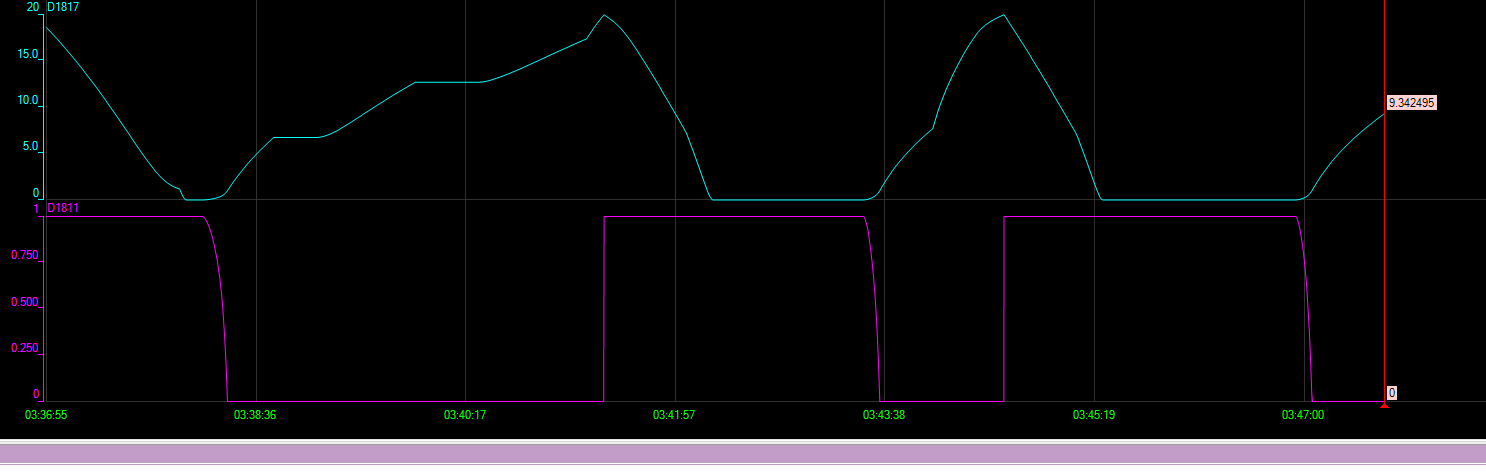
\includegraphics[width=\textwidth, center]{rysunki/SAFETY_MECHANISM_FIGURE_T.png}
	\caption{Wykres prezentuj�cy dzia�anie mechanizmu zabezpieczaj�cego przed uszkodzeniem stanowiska ze zbiornikami na g�rze $H2$, na dole sterowanie $U2$}
	\label{safety_mechanism_figure_t}
\end{figure}

Jak widzimy na powy�szym rysunku (rys. \ref{safety_mechanism_figure_t}), gdy wysoko�� cieczy kt�rego� z wyj�� $H1$ lub $H2$ lub $H3$ jest r�wna $\num{20}$ to odpowiednio otwierane s� zawory $U1$ dla osi�gni�cia wysoko�ci przez $H1$, $U2$ dla osi�gni�cia wysoko�ci przez $H2$ i $U3$ dla osi�gni�cia wysoko�ci przez $H3$. Dzi�ki temu zaw�r odpowiedniego zbiornika, kt�ry osi�ga niebezpieczny poziom cieczy zostanie otworzony.